%\documentclass[10pt]{article}
%\documentclass{sig-alternate}
%\documentclass{llncs}
%\documentclass[twocolumn]{svjour3}
\documentclass[10pt, conference]{IEEEtran}
%\documentclass[10pt, conference, compsocconf]{IEEEtran}
%\documentclass[11pt,draftcls,onecolumn]{IEEEtran}

\usepackage{amsmath}
\usepackage{amssymb}
\usepackage{latexsym}
\usepackage{pifont}
%\usepackage{subfigure}
\usepackage{ifthen}
\usepackage{xspace}
%\usepackage{epic}
%\usepackage{calc}
%\usepackage{verbatim}
%\usepackage{enumerate}
%\usepackage{xspace}
\usepackage{array}
\usepackage{graphicx}
\usepackage{url}
% \usepackage{a4wide}
%\usepackage{extarrows}
\usepackage{color}
\usepackage{booktabs}
\usepackage{bold-extra}
\usepackage{multirow}
%\usepackage{authblk}
%\usepackage{keywords}
%\usepackage{amsthm}
\usepackage{times}
\usepackage{comment}

\let\labelindent\relax
\usepackage{enumitem}

\newtheorem{Prot}{Protocol}
\newtheorem{Thm}{Theorem}
\newtheorem{Def}{Definition}
\newtheorem{Lem}{Lemma}
\newtheorem{Pro}{Proposition}
% \newtheorem{Ex}{Example}
% \newtheorem{Rem}{Remark}
% \newtheorem{Ass}{Assumption}
% \newtheorem{Cor}[Thm]{Corollary}
% \newtheorem{Conj}[Thm]{Conjecture}
% \newtheorem{Prob}[Thm]{Problem}
% \newtheorem{Sol}[Thm]{Solution}

%---Formating---
\renewcommand{\paragraph}{\vspace{3pt}\noindent\textbf}
%\newcommand{\tcodename}{{\fontsize{23}{28}{\scshape{YouCloud}}}\xspace}
%\newcommand{\codename}{{{\scshape{YouCloud}}}\xspace}

%---Algorithms---
\newcommand{\Setup}{\textsf{\textup{Setup}}}
\newcommand{\Update}{\textsf{\textup{Update}}}
\newcommand{\Prove}{\textsf{\textup{Prove}}}
\newcommand{\Verify}{\textsf{\textup{Verify}}}
\newcommand{\Aggregate}{\textsf{\textup{Aggregate}}}
\newcommand{\MK}{\textsf{\textup{MK}}}
\newcommand{\EK}{\textsf{\textup{EK}}}
\newcommand{\CK}{\textsf{\textup{CK}}}

\bibliographystyle{plain}
%\pagestyle{plain}
%\bibliographystyle{IEEEtran}

%--------------------------------------------------------------------

\begin{document}

\title{SoK: On Cloud Resource Accountability}

\maketitle

\begin{abstract}
 This is abstract...
\end{abstract}
       
\section{Introduction} \label{sect:intro}

The concept of cloud computing~\cite{AFG+10}, in large part, is already a reality today.
Computing power is typically {\em centrally} generated in large data centers owned and monopolized by only a few large organizations, e.g., Amazon, Microsoft, and Rackspace, and made available to users via a distributed network.
Centralized clouds may be easier to manage; they are, however, costly to maintain.
Moreover, they may have difficulty in keeping pace with today's and future data growth.
They may also be bandwidth bottlenecks for applications requiring substantial scalability and elasticity~\cite{symform-slide,techrepublic}.

{\em Decentralized clouds} are emerging as attractive alternatives in recent years.
Instead of relying on large and centralized data centers, users harvest the excess computing resources available from Internet-connected computers distributed across the world; in return, the owners of the involved computers earn credits or money (typically in the form of digital currency) proportionate to their contributions.
A few notable examples of such commercial decentralized clouds are Storj~\cite{Storj}, Symform~\cite{Symform}, and MaidSafe~\cite{MaidSafe}.
We note that a decentralized cloud is beyond a multi-cloud, which combines existing centralized clouds into a single virtual cloud storage (e.g., MultCloud~\cite{MultCloud} and Syndicate~\cite{Syndicate}), or a hybrid-cloud, which typically refers to a combination of public and private clouds.
The basic idea of a decentralized cloud here is essentially the same as that of what was traditionally known as volunteer computing, e.g., SETI@home~\cite{Seti@home} and Folding@home~\cite{Folding@home}, or desktop grids~\cite{CKB+07}, e.g., SZTAKI Desktop Grid~\cite{sztaki} and EDGeS~\cite{edges}.
However, a decentralized cloud typically relies on a pricing model, e.g., pay per usage, and the associated accounting and billing services, analogous to those for the existing centralized clouds.
(See~\cite{DP12,MKK13} for further examples and discussions on centralized vs.\ decentralized clouds, and volunteer vs.\ cloud computing.)

- resource usage and billing are top concerns for the majority of IT managers and CIOs 

- existing resource accounting, hard to verify the accuracy and correctness. Also, existing resource metering tools are designed for servers and data centers~\cite{?}.

- The concept of verifiable resource accounting (VRA) was first formalized by Sekar and Maniatis~\cite{SM11}.

- They highlighted that trusted computing can be used to address resource accounting guarantees. However, this cannot be achieved using existing deployed mechanisms. Ideally, a new resource accounting OS or hypervisor should be developed. However, this is not viable given the existing legacy of deployed infrastructure. So, as shown in their subsequent work~\cite{CMP+13}, the only option is to build another layer of lightweight hypervisor on top of existing legacy hypervisors. Nevertheless, there are other challenges remain. For example, such a software-based solution currently can only monitor CPU usage and memory utilization. Also, there's a privacy issue with respect to the cloud provider. It's not clear how the provider's privacy can be protected in terms of their logic and policy of resource allocation (which is usually proprietary).

- the authors acknowledged that what can be done with current TPM technology is only a first step towards an overaching vision. So it may take years to see any deployable and satisfactory TPM-based solution for VRA.

- moreover, it seems infeasible to assume or require each distributed computer in a decentralized cloud model to be equipped with TPM

\paragraph{Goal \& Approach.}
- cryptographic VRA solution can be an appealing immediate and cheaper alternative. In fact, an important point to note is that a cryptographic solution can achieve properties not achievable via TPM, and vice versa. For example, we can provide proofs-of-data-fetch, proofs-of-storage, proofs-of-retrievability, proofs-of-computation, etc., while a TPM-based solution can measure CPU usage and memory utilization. So both approaches can co-exist and complement each other.


\paragraph{Results.}



\section{Current Landscape} \label{sect:current-practice}


\subsection{Threat Model and Trust Assumptions} \label{sect:threat-model}



\subsection{Cloud Service Level Agreements} \label{sect:sla-overview}

- Why are SLAs important?

~\cite{Ahr+10,FMM+13,Kyr13}

\begin{itemize}
 \item Resource availability: Cloud providers typically deliver their services via massively redundant systems to ensure high availability of their services.
 
 \item Data privacy: Data encryption, retention, and deletion. Many organizations have legal requirements that data must be kept for a certain period of time. Some organizations also require that data be deleted after a certain period of time.
 
 \item Hardware erasure and destruction: Improper disposal of hardware may lead to data leakage. If a hard drive fails, the platters of that disk should be zeroed out before the drive is disposed or recycled.

 \item Location: Depending on the kind of data the enterprise is managing on the user's behalf, there might be legal restrictions on the location of the physical server where the data is stored. Cloud vendors can provide an API for determining the location of the physical hardware that delivers the cloud service~\cite{Ahr+10}. For example, many countries prohibit storing personal information about its citizens on any machine outside its borders.
 
 \item Monitoring: The failure to meet the terms of an SLA has financial or legal consequences. So it is vital for the consumer to be able to monitor the performance of the provider. Arguably, the ideal solution has been to let a neutral third-party organization to perform monitoring tasks. This eliminates the conflicts of interest that might occur if the provider report outages at their sole discretion or if the consumer is responsible for proving that an outage occurred. (See \S\ref{sect:sla-monitoring} for discussion on various monitoring techniques and tools.)
 
 \item Auditability: The consumer is liable for any breaches that occur, and thus, it is  vital that the consumer be able to audit the provider's systems and procedures. However, audits are disruptive and expensive. The provider will most likely place limits and charges on them.
 
 \item Maintenance: Cloud providers should inform their consumers about how and when maintenance tasks are carried out.

 \item Resource accounting:
\end{itemize}

- lifecycle of applications and documents, including versioning of applications, the retention and destruction of data 


- we focus on SLA data policies~\cite{Mee12}: data preservation, data redundancy, data location, data privacy.



- Accounting \& Pricing Models~\cite{MMS13}


- currently lack of effective means for a cloud user to verify committed SLAs

\begin{table*}[htb]\centering \footnotesize
\caption{SLA requirements and use case scenarios~\cite{Ahr+10}.}
\label{tab:model-and-requirements}
  \begin{tabular}{lcccccc}
    \toprule
    & $\mathsf{U} \leftrightarrow \mathsf{C}$ & $\mathsf{E} \leftrightarrow \mathsf{C} \leftrightarrow \mathsf{U}$ & $\mathsf{E} \leftrightarrow \mathsf{C}$ & $\mathsf{E} \leftrightarrow \mathsf{C} \leftrightarrow \mathsf{E}$ & Private cloud & Hybrid cloud \\
    \midrule
    Data encryption &&& \cmark &&& \\
    Privacy & \cmark & \cmark & \cmark & \cmark & \cmark & \cmark \\
    Data retention \& deletion &&& \cmark & \cmark && \cmark \\
    Hardware erasure \& destruction &&& \cmark & \cmark && \cmark \\
    Regulatory compliance & \cmark & \cmark & \cmark & \cmark & \cmark & \cmark \\
    Transparency & \cmark & \cmark & \cmark & \cmark & \cmark & \cmark \\
    Certification & \cmark & \cmark & \cmark & \cmark & \cmark & \cmark \\
    Terminology for PKIs &&& \cmark & \cmark & \cmark & \cmark \\
    Metrics & \cmark & \cmark & \cmark & \cmark & \cmark & \cmark \\
    Auditability & \cmark &&&&&\\
    Monitoring & \cmark & \cmark & \cmark & \cmark & \cmark & \cmark \\
    Machine-readable SLAs &&&& \cmark && \\
   \bottomrule
   \multicolumn{7}{l}{\scriptsize Notation: $\mathsf{U}$ denotes end user; $\mathsf{E}$ denotes enterprise; $\mathsf{C}$ denotes cloud; $\leftrightarrow$ denotes interactivity.}
  \end{tabular}
\end{table*}



\begin{table}[htb]\centering \footnotesize
\caption{SLA comparison between cloud providers~\cite{Bas12}.}
\label{tab:sla-comparison}
  \begin{tabular}{lccc}
    \toprule
    & Amazon & Azure & Rackspace \\
    \midrule
    Service guarantee &&& \\
    Scheduled maintenance &&& \\
    OS/software patches &&& \\
    Service guarantee time period &&& \\
    Service credit &&& \\
    Violation reporting onus &&& \\
    Violation incident reporting &&& \\
    Violation claim filing &&& \\
    SLA publish date &&& \\
   \bottomrule
  \end{tabular}
\end{table}


\subsection{Accounting and Pricing Models} \label{sect:accounting}


\subsection{Monitoring} \label{sect:sla-monitoring}

- service level management via monitoring and measuring the performance of the provided services are key to determining if a SLA is met.
- SLM allows a cloud provider to make decisions based on its business objectives and technical realities. For example, the cloud provider could reallocate bandwidth or bring more physical hardware online when the throughput for a service is not meeting a consumer's requirements.
- From the consumer's perspective, SLM helps in making decisions (possibly in an automated manner) about the way it uses cloud services~\cite{Ahr+10}.


- motivations for monitoring~\cite{DLN12,EFN+12}

- review of existing cloud service monitoring tools~\cite{ABD+13,FEH+14}

- monitoring metrics: throughput, load balancing, elasticity, agility, customer service response time, etc. These are not difficult to measure.

\begin{table*}[htb]\centering \footnotesize
\caption{Existing commercial and open-source cloud monitoring tools and their key properties \& features~\cite{FEH+14}.}
\label{tab:monitoring-tools}
  \begin{tabular}{lccccccc}
     \toprule
     & Amazon & AzureWatch~\cite{AzureWatch} & Rackspace & CA Nimsoft & Monitis~\cite{Monitis} & Nagios~\cite{Nagios} & PCMONS~\cite{Pcmons} \\
     & CloudWatch~\cite{CloudWatch} && Cloud Monitor~\cite{RackspaceCloudMonitoring} & Monitor~\cite{Nimsoft} &&& \\
     \midrule
     Scalability & \cmark & \cmark & \cmark & \cmark &\cmark && \\
     Portability &&& Limited & \cmark & \cmark & Limited & \\
     Multi-tenancy & \cmark & \cmark & \cmark & \cmark && \cmark & \\
     Interoperability &&&&&&& \cmark \\
     Customizability & \cmark & \cmark & \cmark & \cmark & \cmark & \cmark & \cmark \\
     Resource usage metering & \cmark & \cmark & \cmark & \cmark & \cmark & \cmark & \cmark \\
     {\bf Verifiable measuring} &&&&&&& \\
     Service load monitoring & \cmark & \cmark & \cmark & \cmark & \cmark & \cmark & \cmark \\
     {\bf Service PKI monitoring} &&&&&&& \\
     Risk assessment & \cmark & \cmark & \cmark & \cmark & Limited & \cmark & \cmark \\
     Security breach monitoring & \cmark & \cmark & \cmark & \cmark && \cmark & \\
    \bottomrule
  \end{tabular}
\end{table*}

\subsection{Auditability} \label{sect:auditability}

Existing major cloud providers (e.g., Amazon, Rackspace, and Microsoft) leave the burden of detecting SLA violation to the customer~\cite{Bas12}.

- verify based on well-defined metrics, Service Measurement Index (SMI)

CloudProof~\cite{PLM+11}


- Most public cloud services offer a non-negotiable SLA. With these providers, a consumer whose requirements are not met can either: (i) accept a credit towards next month's bill, or (ii) stop using the service.

- To provide services cost-effectively, a cloud will manage the pool of hardware resources for resource efficiency; one of the strategies that a cloud provider employs during periods of reduced consumer demand is to power off unused components. Whether for power management, or for hardware refresh, migration of customer workloads (data storage and processing) from one physical computer to another physical computer is a key strategy that allows a provider to refresh hardware or consolidate workloads without inconveniencing consumers~\cite{BGP+12}.



\section{Emerging Trends} \label{sect:new-trends}

The concept of verifiable resource accounting (VRA) was first formalized by Sekar and Maniatis~\cite{SM11}.
Here, verifiability aims to give cloud customers assurance about two questions:
\begin{itemize}
 \item Did I consume what I was charged?
 \item Should I have consumed what I was charged?
\end{itemize}
The first question is about the accuracy of the consumption vector, e.g., CPU time, in/out network bandwidth, storage, etc. The cloud provider should not be able to charge a customer with resources it did not expend on her behalf. The second question concerns itself with the efficiency of the provider's infrastructure, e.g., with respect to scheduling and provisioning. If the provider erroneously used 1 GB of memory for a task instead of 1 MB, it should arguably not able to pass on the cost of its inefficiency to its customer.

It was envisioned in [SM11] that verifiable resource accounting can be realized in the following operating model: the provider generates a consumption report describing what resources it thinks a customer has consumed for a task. The customer then is able to check either by herself or via an independent component or party the validity of the consumption report. 

\subsection{Cryptographic Audits} \label{sect:crypto-audits}


- cryptographic VRA solution can be an appealing immediate and cheaper alternative. In fact, an important point to note is that a cryptographic solution can achieve properties not achievable via TPM, and vice versa. For example, we can provide proofs-of-data-fetch, proofs-of-storage, proofs-of-retrievability, proofs-of-computation, etc., while a TPM-based solution can measure CPU usage and memory utilization. So both approaches can complement each other.

\subsection{Trusted Computing} \label{sect:trusted-computing}

Chen et al.~\cite{CMP+13} proposed an instantiation of a verification mechanism via trusted trusted computing components. 
Their solution leverages advances in nested virtualization to build a trusted ``observer'' for monitoring and reporting resource use, e.g., CPU and memory usage.

They highlighted that trusted computing can be used to address resource accounting guarantees. However, this cannot be achieved using existing deployed mechanisms. Ideally, a new resource accounting OS or hypervisor should be developed. However, this is not viable given the existing legacy of deployed infrastructure. So, as shown in~\cite{CMP+13}, the only option is to build another layer of lightweight hypervisor on top of existing legacy hypervisors. Nevertheless, there are other challenges remain. For example, such a software-based solution currently can only monitor CPU usage and memory utilization. Also, there's a privacy issue with respect to the cloud provider. It's not clear how the provider's privacy can be protected in terms of their logic and policy of resource allocation (which is usually proprietary).

- the authors acknowledged that what can be done with current TPM technology is only a first step towards an overaching vision. So it may take years to see any deployable and satisfactory TPM-based solution for VRA.

\subsection{Others} \label{sect:other-trends}


~\cite{HDT+14,ZYS+14}

In THEMIS~\cite{PHC+13}, a trusted third party acting as a notary between the client and the cloud provider is used to verify the client’s resource consumption. It relies on digital signatures to protect the integrity and non-repudiability of billing transactions associated with resources consumed by the client. Billing statements issued by the cloud provider is compared against information obtained via a SLA monitoring module enhanced with TPM technology.

A peer-to-peer billing and accounting system for the cloud called BitBill was recently proposed~\cite{CC14} to remove assumptions relying on a trusted component or third party for verification purposes. It adopts a Bitcoin-like decentralized verification mechanism. That is, the trusted third party is replaced by a global log of all the resource provision and usage of all clients and providers. Every billable event has to be signed and broadcast, analogous to that of Bitcoin. The clients and providers verify and agree on a log of events with the help of other clients from the same resource pool. To prevent malicious nodes from forging false events, a similar proof-of-work technique is used such that the rate of announcement can be controlled.

- automating detection of SLAs violations~\cite{ENC+12,EBM+13}

\section{Technical Overview} \label{sect:techniques}

\subsection{Storage}

Early proof-of-storage systems were proposed by Golle, Jarecki, and Mironov~\cite{GJM02}, Deswarte, Quisquater, and Sa\"{\i}dane~\cite{DQS03}, Filho and Barreto~\cite{FB06}, and Schwarz and Miller~\cite{SM06}.
However, these proposals lacked a formal security model and analysis.
Juels and Kaliski~\cite{JK07}, Naor and Rothblum~\cite{NR09} considered the first formal models in the context of authenticators and proofs of retrievability (POR), respectively.
Subsequently, a series of improvements have been proposed, for example, in terms of public verifiability~\cite{AKK09,ABC+11}, compactness of proofs~\cite{SW13}, support for dynamic data update~\cite{ADM+08,EKP+09,WWL+09,SDJ+12,CKW13,SSP13}, replication~\cite{CKB+08}, and security against a fully Byzantine adversarial model~\cite{BJO09a}.

There also exist proposals distributed proof-of-storage systems.
Bowers, Juels, and A. Oprea~\cite{BJO09b} proposed HAIL, in which files are divided in segments and stored across a collection of distributed servers.
They showed that the integrity and availability of files can be realized using file authentication techniques and integrity-protected error-correcting code in an interactive and synchronous manner among the distributed servers.
Zhu et al.~\cite{ZHA+12} considered a distributed proof-of-data-possession (PDP) system in a multi-cloud model, which requires a trusted third party to store public parameters used for proof verification.
On the other hand, Etemad and K{\"u}p\c{c}{\"u}~\cite{EK13} proposed a distributed and replicated dynamic PDP system which is transparent from the user's viewpoint (in terms of the internal architecture of the cloud provider).
In very recent development, Miller et al.~\cite{MJS+14} show that a distributed POR system can be adapted for mining Bitcoin (instead of using computational resources).

\paragraph{Possession.}

\paragraph{Retrievability.}

\paragraph{Redundancy.}




\subsection{Computation}

\paragraph{Correctness.}

\paragraph{Effort.}

[Proof systems]
Various general-purpose proof systems, pioneered by the work of Babai~\cite{Bab85} and Goldwasser et al.~\cite{GMR89}, have been proposed for verifying computation of arbitrary functions.
Proposals in this line of research are largely theoretical.
However, recent promising results on more efficient proof systems, e.g., Pinocchio~\cite{PHG+13} and TrueSet~\cite{KPP+14}, give a glimpse of hope for possible practical deployment of these systems.
Nevertheless, further refinements and research are required before they become truly practical.

%\paragraph{Interactive Proofs.}
Earlier theoretical proof systems involve interaction between a prover and a verifier.
Interactive proofs, such as~\cite{LFK+92,Sha92}, allow the prover to probabilistically convince the verifier of the truth of any function computable in polynomial time.
Typically the prover runs in super-polynomial time, while the verifier runs in polynomial time.
Nevertheless, Goldwasser et al.~\cite{GKR08} showed that for computation of small space or depth, it is possible to reduce the prover complexity for interactive proofs to polynomial time, and the verifier complexity to almost linear time.  

From interactive proof systems, one can derive {\em probabilistically checkable proofs} (PCPs), allowing the verifier to randomly check only a small fraction of the proof, e.g., a constant number of bits of the proof for NP languages.
However, this typically requires the prover to provide a long PCP (of polynomial length) to the verifier.
Kilian~\cite{Kil92} and Micali~\cite{Mic94} showed that {\em interactive arguments} (aka computationally sound proofs), in which the prover is assumed to be computationally bounded, can be used to alleviate such an issue.
Particularly, they gave constant-round protocols with a polynomial-time prover and an almost linear-time verifier, assuming the existence of collision-resistant functions.

A series of recent work has considerably improved the efficiency of interactive proof-based verifiable computation, see for example~\cite{CMT12,SMB+12,SVP+12,TRM+12,VSB+13}.
However, these proposals are still not practical.

%\paragraph{Non-interactive Proofs.}
Micali~\cite{Mic94} also suggested that a non-interactive proof system (with roughly similar efficiency to that of the interactive version) is possible in the random oracle model~\cite{BR93}.
However, the random oracle heuristic is known to be unsound in general~\cite{CGH04}.
More recently, Goldwasser et al.~\cite{GKR08} showed that interactive proofs for small-depth computation can be converted into non-interactive arguments, assuming the existence of single-server private information retrieval (PIR)~\cite{CKG+98}.
Nevertheless, such arguments are applicable to only a restricted class of functions.

Gennaro et al.~\cite{GGP10} recently showed that it is possible to verify any arbitrary computation by increasing the verifier offline complexity and making use of fully homomorphic encryption (FHE)~\cite{Gen09}.
They observed that Yao's garbled circuit construction~\cite{Yao82} provides a ``one-time'' verifiable computation, in addition to allowing secure two-party computation.
Hence, Yao's construction can be adapted to allow a client to outsource the computation of a function to a worker, while allowing the client to verify the correctness of the output of the computation.
However, reusing the same circuit for different input is insecure, and thus, Gennaro et al.\ proposed the combined use of a garbled circuit and FHE, such that the circuit is evaluated by the worker in an encrypted domain.
This way, the labels associated with the bits of client's input is not leaked and can be reused many times.
The use of FHE ensures input and output privacy for the client.
To evaluate a function $F:\{0,1\}^n \to \{0,1\}^m$, which can be described by a Boolean circuit $C$, the Gennaro et al.\ VC scheme requires one-time (offline)  preprocessing step that takes $O(|C|)$ time, i.e., comparable to computing the function from scratch.
However, the one-time cost can be amortized over many executions on different input choices for the same function.
At the online stage, the client runs in linear time, that is, input preparation takes $O(n)$ time and output verification takes $O(m)$ time.
On the other hand, the worker takes $O(|C|)$ to compute the function for the client.
Subsequently Chung et al.~\cite{CKV10} proposed a VC scheme (also with input and output privacy) which reduces the preprocessing cost to $O(\log(|C|))$, but requiring an additional round of communication between the client and the worker.

However, FHE-based VC schemes have an inherent limitation.
The output of the verification check performed by the client must not be revealed to the worker; otherwise a malicious worker may learn a bit of information about the labels of the evaluated garbled circuit.
This is known as the ``rejection problem''.\footnote{A malicious cloud that is able to observe the result of the verification procedure, i.e., accept/reject decision, on polynomially many inputs can eventually break the soundness of the scheme~\cite{PRV12}.}
Various approaches have been proposed to address this, such as public VC (supporting public delegatability and verifiable)~\cite{PRV12,PST13}, memory delegation~\cite{CKL+11}, combined PCP and PIR techniques~\cite{BCC+12}, combined FHE and function encryption~\cite{BF12}.

Parno et al.~\cite{PHG+13} recently proposed Pinocchio, a system for public verifiable general-purpose computation with orders of magnitude efficiency improvement over previous proposals.
Their solution make use of {\em quadratic programs}~\cite{GGP+13}, which allows compact encoding of computation from an associated arithmetic or Boolean circuit, in order to speed up proof generation and verification.
The key setup and proof generation require cryptographic effort linear in the size of the original computation, and verification requires time linear in the size of the input and output.
Kosba et al.~\cite{KPP+14} proposed {\sc TrueSet}, which further improves the efficiency of Pinocchio.
Their core idea is to model computation as a {\em set circuit}, i.e., circuit on polynomials, which can be encoded as quadratic polynomial programs.
This is then combined with {\em succinct non-interactive argument of knowledge} (SNARK)~\cite{GGP+13} for polynomial circuits to achieve input-specific running time during key setup and proof generation.
{\sc TrueSet} supports arbitrary computation tasks since the set circuit supports intersection, union, and difference gates.
However, both Pinocchio and {\sc TrueSet} do not preserve input and output privacy.

There also exist other efficient VC solutions but supporting smaller classes of functions, polynomials and set operations, see for example~\cite{BGV11,PTT11,FG12}.
Publicly verifiable set operations over outsourced and {\em authenticated} datasets are considered in~\cite{CPP+14}.

Recently Fiore, Gennaro, and Pastro~\cite{FGP14} developed a new homomorphic hashing technique that allows efficient verifiable computation...

------------

There exist several reasonably efficient and practical methods for verifying general secure computation on data outsourced by a client to one or multiple workers (or servers).

[Replication]
One natural and simple way for the client to verify the correctness of computation is to request multiple workers to execute its program on the same dataset. The client then takes the plurality value of the results from the workers to be the correct answer. As long as a majority of the workers are honest, the client gets the correct answer. In case there is inconsistency, the client can execute the program itself. Typically, the client and the workers sign all messages exchanged between them. This is to prevent sybil and impersonation attacks, for example.

The need for an honest majority of workers can be obviated using refereed delegation of computation~\cite{CRR11}. In this computation model, the client requests for the result of a function from two (or more) workers. In case of inconsistency, the client can efficiently determine the true claim as long as there is at least one honest worker. Here, the client acts as a ``referee'' and is not required to perform the verification itself. The overhead (in the event of inconsistency or dispute) is poly-logarithmic in the size of the computation. It has been shown in~\cite{CRR11} that, for some parameters, one gets an 8x slowdown in a program for computing the determinant of a given matrix.

Alternatively, the client can establish a contractual agreement with two (or more) workers in one of the following two ways~\cite{NK12}:
\begin{itemize}
 \item If the client asks for computation results from both workers, and the results do not match, both workers pay a penalty to the client, and return the money paid for the computation as well.
 \item If the client asks for computation results from both workers, and the results do not match, the client performs a potentially costly audit of the computation. Each worker whose result does not match the result given by the client's audit pays a fine to the client.
\end{itemize}
The above two agreements can be proved in a game-theoretic model that they have individually rational and incentive compatible equilibrium, assuming the workers behave honestly. 
It was recently shown in~\cite{CKP14} that optimal results (in terms of the client's expected costs) can still be achieved even when considering side-channel information and collusion among workers.

Clearly, a limitation of the replication method is the need for at least two workers for any computational tasks. However, in return, the client is guaranteed of detecting any cheating worker.

[Random Spot-checking]
Another common approach is to insert fake, random items at random positions when forming a computational task for a worker~\cite{GM01,JK07}. The fake items need to be chosen only once for all tasks. Upon job completion, the client checks if the returned results corresponding to the fake items are as expected. The complexity of verification overhead is $O(n)$ for $n$ fake items, where n is chosen sufficiently large for achieving high probability of cheating detection. It was recently shown in~\cite{BZF13} that for secure (privacy-preserving) and verifiable outsourcing of Hamming distance computations, the worker's computational overhead increases only moderately, by roughly 10-24\% for different sizes of datasets after insertion of fake items. On the other hand, the client's preparation and verification overhead is roughly 8 seconds for a dataset of 8,000 items.

The spot-checking approach may be cheaper than using replication, with slightly weaker (probabilistic) guarantee of cheating detection.

[Obfuscation of Code]
One can also use code obfuscation techniques, e.g., to insert checkable state points in computational tasks, such that the worker is able to produce proofs of execution comprising a sequence of state points, which can be verified by the worker~\cite{Hoh98, MWR99}.

[Trusted Hardware]
The client may also use trusted hardware, e.g., tamper-proof co-processor, on the server to prove the correctness of the computation~\cite{SPD05}. This is somewhat conceptually similar to relying on a weak trusted third party, i.e., hardware manufacturer.

Kumaresan and Bentove~\cite{KB14} recently proposed a model of incentivizing correct computation using Bitcoin. 


\subsection{Data Transfer}

Verifiable Content Distribution. It was shown in~\cite{KFM04} that verification of erasure-encoded data blocks in P2P-CDNs can be performed on-the-fly, i.e., recipients can verify the integrity of check blocks immediately as each data block is downloaded. Such a scheme can be constructed based on a homomorphic hash function.

File sharing or content distribution is commonly done over a peer-to-peer (P2P) network. However, a fundamental problem in a P2P network is the so-called ``free riders'' problem, i.e., users who use the services provided by others but do not provide any services to their peers. 
Motivated by this problem, Golle, Jarecki, and Mironov~\cite{GJM02} introduced two cryptographic primitives:
communication-enforcing signature (CES), which enforces ``proofs-of-download'' or ``pay-for-bandwidth'' in the context of P2P content distribution networks (P2P-CDNs);
storage-enforcing commitment (SEC), which enforces ``proofs-of-storage'' or ``proofs-of-data-possession''.
Standard signatures are not adequate as proofs-of-download, since the hash-and-sign paradigm implies that knowledge of the digest of a message is sufficient to sign the whole message. Hence, a dishonest user can save on bandwidth by exchanging only the hashes of requested content and claim credit for content she has never downloaded. CES works in such a way that the signer can only sign a message after exchanging at least as much data with the requester as would be required to send the entire message. On the other hand, SEC is based on a standard commitment scheme with the additional property that the party holding a commitment can ask the party that committed itself to a message to prove that it is still in the possession of the message.

Subsequently in~\cite{FB06}, a CES scheme in a stronger security model, which assumes both uploaders and downloaders are untrusted, was proposed. A SEC scheme with smaller public key size was also proposed.



\subsection{Location}

~\cite{WSA+12}

\subsection{Isolation}

~\cite{WSJ+12,WSJ+13,WSJ+14}

\subsection{Space}

There also exist primitives to enable a client to verify if the cloud has the requested amount of memory space~\cite{ABF13} and disk space~\cite{DFK+13}.

\subsection{Erasure}

~\cite{PT10}

\section{Review of TPM-based Mechanisms} \label{sect:tpm}
\section{Analysis and Discussion} \label{sect:analysis}


\subsection{Security}


\subsection{Practicality}
\section{Problem \& Solution} \label{sect:overview}

\subsection{Problem Definition} \label{sect:problem}

We consider a data owner (client) storing her data in encrypted form on a server, possibly residing on a centralized cloud or a peer-to-peer (P2P) network.
The owner may run computational intensive tasks over the encrypted data.
Instead of performing tasks on the server itself, the owner delegates them to multiple workers residing on a decentralized cloud. 
Each worker fetches its portion of the required dataset from the server, performs the requested computation, and returns the results to the server.
The owner can then, at her discretion, download and verify the results.
The worker is financially rewarded if the verification of the returned results passes through.
This is illustrated in Figure~\ref{fig:model}.
In this work, we ask the question of {\em how can the owner securely and efficiently verify the resource consumption of each worker without relying on a trusted third party or any trusted hardware component}?

\begin{figure}[h!]\centering
  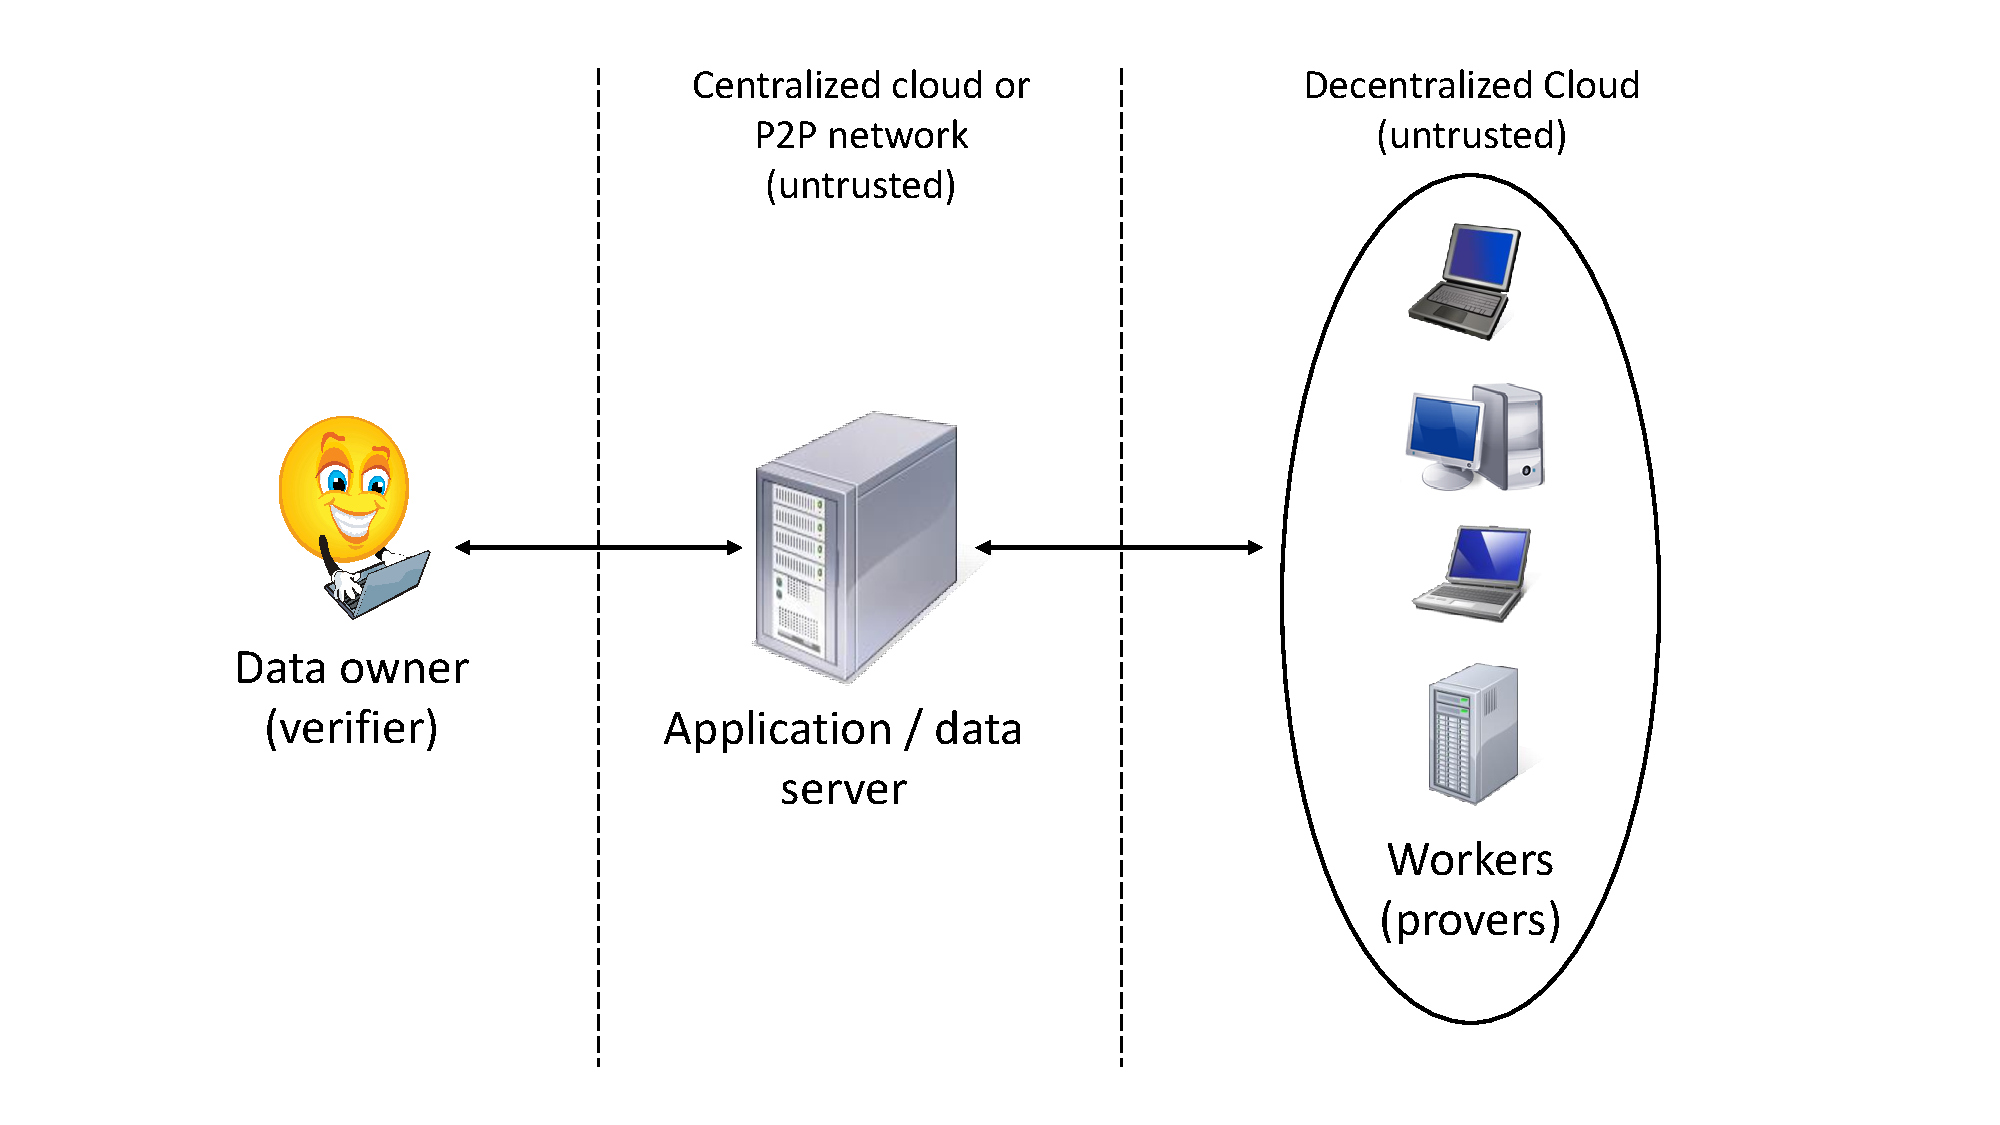
\includegraphics[scale=0.30]{model.pdf}
  \caption{Outsource of data and computation to a decentralized cloud.}
  \label{fig:model}
\end{figure}

Our decentralized cloud setting has the following distinctive characteristics in comparison to centralized cloud settings previously considered:
\begin{itemize}
 \item A data owner distributes her datasets and delegate computational tasks to a decentralized and heterogeneous computing environment.
 \item There exists an intermediate party, i.e., application/data server, which facilitates delegation and distribution of datasets and computational tasks.
 \item The owner can dynamically update her datasets stored on the server, but the data delegated to workers is assumed to be static.
 \item The owner's dataset is stored on the server over an extended period of time, but any data distributed to the worker is only temporarily stored and deleted upon the completion of the assigned task.
\end{itemize}

We note that the introduction of a centralized entity to facilitate distribution of tasks is necessary in our decentralized infrastructure.
In fact, BOINC~\cite{And04} also relies on centralized data and application servers to distribute tasks within a volunteer computing network, and BitTorrent~\cite{Coh03} uses a trusted, centralized tracker to coordinate activities within a P2P network.

\paragraph{Threat Model.}
However, each worker is assumed to be untrusted and they may deviate from the intended computation for various reasons, e.g., to save on computational cost. 
%It is essential, therefore, for the client to be able to verify the correctness of the computation. 
On the other hand, the worker may not trust the data owner either, in the sense that the worker may not be rewarded even if it has completed the computation and proved the correctness of the computation.


\subsection{Challenges} \label{sect:challenges}

\paragraph{Proofs of Data Fetch.}
- One challenge is how to reduce the number of verifications required over multiple workers (currently a prover can convince a verifier with a constant number of challenges/responses for each file). 

- Another issue is that if the worker knows in advance the positions of the challenge data blocks, then it simply downloads only those blocks. Existing POR systems do not encounter such a problem because a file is stored for a relatively extended period of time and different challenges on different positions may be issued to the worker. This forces the worker to download the entire file.

- During update of elements of the dataset, how can the owner update her local state information (used for verifying resource consumption) in an efficient manner?

\paragraph{Proofs of Computation.}
- why POC is sufficient for some applications compared to checking the correctness of computation? (However, for some applications, it may be easier to verify the correctness of computation, which could imply both PDF and POC.)

\paragraph{Fairness.}



\subsection{Solution Overview} \label{sect:solution}


\section{Open Problems} \label{sect:open-problems}


\subsection{Efficiency}


\subsection{Generality}

\subsection{Fairness}
\section{Related Work} \label{sect:related-work}


Recent surveys:
- verifiable computing~\cite{WB13} 
- general verifiable cloud services~\cite{BCC+13}, 
- cloud monitoring~\cite{ABD+13,FEH+14}

-----------------------------

\subsection{Storage}

Early proof-of-storage systems were proposed by Golle, Jarecki, and Mironov~\cite{GJM02}, Deswarte, Quisquater, and Sa\"{\i}dane~\cite{DQS03}, Filho and Barreto~\cite{FB06}, and Schwarz and Miller~\cite{SM06}.
However, these proposals lacked a formal security model and analysis.
Juels and Kaliski~\cite{JK07}, Naor and Rothblum~\cite{NR09} considered the first formal models in the context of authenticators and proofs of retrievability (POR), respectively.
Subsequently, a series of improvements have been proposed, for example, in terms of public verifiability~\cite{AKK09,ABC+11}, compactness of proofs~\cite{SW13}, support for dynamic data update~\cite{ADM+08,EKP+09,WWL+09,SDJ+12,CKW13,SSP13}, replication~\cite{CKB+08}, and security against a fully Byzantine adversarial model~\cite{BJO09a}.

There also exist proposals distributed proof-of-storage systems.
Bowers, Juels, and A. Oprea~\cite{BJO09b} proposed HAIL, in which files are divided in segments and stored across a collection of distributed servers.
They showed that the integrity and availability of files can be realized using file authentication techniques and integrity-protected error-correcting code in an interactive and synchronous manner among the distributed servers.
Zhu et al.~\cite{ZHA+12} considered a distributed proof-of-data-possession (PDP) system in a multi-cloud model, which requires a trusted third party to store public parameters used for proof verification.
On the other hand, Etemad and K{\"u}p\c{c}{\"u}~\cite{EK13} proposed a distributed and replicated dynamic PDP system which is transparent from the user's viewpoint (in terms of the internal architecture of the cloud provider).
In very recent development, Miller et al.~\cite{MJS+14} show that a distributed POR system can be adapted for mining Bitcoin (instead of using computational resources).

\paragraph{Integrity.}

\paragraph{Consistency.}

\paragraph{Possession.}

\paragraph{Retrievability.}

\paragraph{Redundancy.}




\subsection{Computation}

\paragraph{Correctness.}

\paragraph{Effort.}

[General proof of work]

[Proof systems]
Various general-purpose proof systems, pioneered by the work of Babai~\cite{Bab85} and Goldwasser et al.~\cite{GMR89}, have been proposed for verifying computation of arbitrary functions.
Proposals in this line of research are largely theoretical.
However, recent promising results on more efficient proof systems, e.g., Pinocchio~\cite{PHG+13} and TrueSet~\cite{KPP+14}, give a glimpse of hope for possible practical deployment of these systems.
Nevertheless, further refinements and research are required before they become truly practical.

%\paragraph{Interactive Proofs.}
Earlier theoretical proof systems involve interaction between a prover and a verifier.
Interactive proofs, such as~\cite{LFK+92,Sha92}, allow the prover to probabilistically convince the verifier of the truth of any function computable in polynomial time.
Typically the prover runs in super-polynomial time, while the verifier runs in polynomial time.
Nevertheless, Goldwasser et al.~\cite{GKR08} showed that for computation of small space or depth, it is possible to reduce the prover complexity for interactive proofs to polynomial time, and the verifier complexity to almost linear time.  

From interactive proof systems, one can derive {\em probabilistically checkable proofs} (PCPs), allowing the verifier to randomly check only a small fraction of the proof, e.g., a constant number of bits of the proof for NP languages.
However, this typically requires the prover to provide a long PCP (of polynomial length) to the verifier.
Kilian~\cite{Kil92} and Micali~\cite{Mic94} showed that {\em interactive arguments} (aka computationally sound proofs), in which the prover is assumed to be computationally bounded, can be used to alleviate such an issue.
Particularly, they gave constant-round protocols with a polynomial-time prover and an almost linear-time verifier, assuming the existence of collision-resistant functions.

A series of recent work has considerably improved the efficiency of interactive proof-based verifiable computation, see for example~\cite{CMT12,SMB+12,SVP+12,TRM+12,VSB+13}.
However, these proposals are still not practical.

%\paragraph{Non-interactive Proofs.}
Micali~\cite{Mic94} also suggested that a non-interactive proof system (with roughly similar efficiency to that of the interactive version) is possible in the random oracle model~\cite{BR93}.
However, the random oracle heuristic is known to be unsound in general~\cite{CGH04}.
More recently, Goldwasser et al.~\cite{GKR08} showed that interactive proofs for small-depth computation can be converted into non-interactive arguments, assuming the existence of single-server private information retrieval (PIR)~\cite{CKG+98}.
Nevertheless, such arguments are applicable to only a restricted class of functions.

Gennaro et al.~\cite{GGP10} recently showed that it is possible to verify any arbitrary computation by increasing the verifier offline complexity and making use of fully homomorphic encryption (FHE)~\cite{Gen09}.
They observed that Yao's garbled circuit construction~\cite{Yao82} provides a ``one-time'' verifiable computation, in addition to allowing secure two-party computation.
Hence, Yao's construction can be adapted to allow a client to outsource the computation of a function to a worker, while allowing the client to verify the correctness of the output of the computation.
However, reusing the same circuit for different input is insecure, and thus, Gennaro et al.\ proposed the combined use of a garbled circuit and FHE, such that the circuit is evaluated by the worker in an encrypted domain.
This way, the labels associated with the bits of client's input is not leaked and can be reused many times.
The use of FHE ensures input and output privacy for the client.
To evaluate a function $F:\{0,1\}^n \to \{0,1\}^m$, which can be described by a Boolean circuit $C$, the Gennaro et al.\ VC scheme requires one-time (offline)  preprocessing step that takes $O(|C|)$ time, i.e., comparable to computing the function from scratch.
However, the one-time cost can be amortized over many executions on different input choices for the same function.
At the online stage, the client runs in linear time, that is, input preparation takes $O(n)$ time and output verification takes $O(m)$ time.
On the other hand, the worker takes $O(|C|)$ to compute the function for the client.
Subsequently Chung et al.~\cite{CKV10} proposed a VC scheme (also with input and output privacy) which reduces the preprocessing cost to $O(\log(|C|))$, but requiring an additional round of communication between the client and the worker.

However, FHE-based VC schemes have an inherent limitation.
The output of the verification check performed by the client must not be revealed to the worker; otherwise a malicious worker may learn a bit of information about the labels of the evaluated garbled circuit.
This is known as the ``rejection problem''.\footnote{A malicious cloud that is able to observe the result of the verification procedure, i.e., accept/reject decision, on polynomially many inputs can eventually break the soundness of the scheme~\cite{PRV12}.}
Various approaches have been proposed to address this, such as public VC (supporting public delegatability and verifiable)~\cite{PRV12,PST13}, memory delegation~\cite{CKL+11}, combined PCP and PIR techniques~\cite{BCC+12}, combined FHE and function encryption~\cite{BF12}.

Parno et al.~\cite{PHG+13} recently proposed Pinocchio, a system for public verifiable general-purpose computation with orders of magnitude efficiency improvement over previous proposals.
Their solution make use of {\em quadratic programs}~\cite{GGP+13}, which allows compact encoding of computation from an associated arithmetic or Boolean circuit, in order to speed up proof generation and verification.
The key setup and proof generation require cryptographic effort linear in the size of the original computation, and verification requires time linear in the size of the input and output.
Kosba et al.~\cite{KPP+14} proposed {\sc TrueSet}, which further improves the efficiency of Pinocchio.
Their core idea is to model computation as a {\em set circuit}, i.e., circuit on polynomials, which can be encoded as quadratic polynomial programs.
This is then combined with {\em succinct non-interactive argument of knowledge} (SNARK)~\cite{GGP+13} for polynomial circuits to achieve input-specific running time during key setup and proof generation.
{\sc TrueSet} supports arbitrary computation tasks since the set circuit supports intersection, union, and difference gates.
However, both Pinocchio and {\sc TrueSet} do not preserve input and output privacy.

There also exist other efficient VC solutions but supporting smaller classes of functions, polynomials and set operations, see for example~\cite{BGV11,PTT11,FG12}.
Publicly verifiable set operations over outsourced and {\em authenticated} datasets are considered in~\cite{CPP+14}.

Recently Fiore, Gennaro, and Pastro~\cite{FGP14} developed a new homomorphic hashing technique that allows efficient verifiable computation...

------------

There exist several reasonably efficient and practical methods for verifying general secure computation on data outsourced by a client to one or multiple workers (or servers).

[Replication]
One natural and simple way for the client to verify the correctness of computation is to request multiple workers to execute its program on the same dataset. The client then takes the plurality value of the results from the workers to be the correct answer. As long as a majority of the workers are honest, the client gets the correct answer. In case there is inconsistency, the client can execute the program itself. Typically, the client and the workers sign all messages exchanged between them. This is to prevent sybil and impersonation attacks, for example.

The need for an honest majority of workers can be obviated using refereed delegation of computation~\cite{CRR11}. In this computation model, the client requests for the result of a function from two (or more) workers. In case of inconsistency, the client can efficiently determine the true claim as long as there is at least one honest worker. Here, the client acts as a ``referee'' and is not required to perform the verification itself. The overhead (in the event of inconsistency or dispute) is poly-logarithmic in the size of the computation. It has been shown in~\cite{CRR11} that, for some parameters, one gets an 8x slowdown in a program for computing the determinant of a given matrix.

Alternatively, the client can establish a contractual agreement with two (or more) workers in one of the following two ways~\cite{NK12}:
\begin{itemize}
 \item If the client asks for computation results from both workers, and the results do not match, both workers pay a penalty to the client, and return the money paid for the computation as well.
 \item If the client asks for computation results from both workers, and the results do not match, the client performs a potentially costly audit of the computation. Each worker whose result does not match the result given by the client's audit pays a fine to the client.
\end{itemize}
The above two agreements can be proved in a game-theoretic model that they have individually rational and incentive compatible equilibrium, assuming the workers behave honestly. 
It was recently shown in~\cite{CKP14} that optimal results (in terms of the client's expected costs) can still be achieved even when considering side-channel information and collusion among workers.

Clearly, a limitation of the replication method is the need for at least two workers for any computational tasks. However, in return, the client is guaranteed of detecting any cheating worker.

[Random Spot-checking]
Another common approach is to insert fake, random items at random positions when forming a computational task for a worker~\cite{GM01,JK07}. The fake items need to be chosen only once for all tasks. Upon job completion, the client checks if the returned results corresponding to the fake items are as expected. The complexity of verification overhead is $O(n)$ for $n$ fake items, where n is chosen sufficiently large for achieving high probability of cheating detection. It was recently shown in~\cite{BZF13} that for secure (privacy-preserving) and verifiable outsourcing of Hamming distance computations, the worker's computational overhead increases only moderately, by roughly 10-24\% for different sizes of datasets after insertion of fake items. On the other hand, the client's preparation and verification overhead is roughly 8 seconds for a dataset of 8,000 items.

The spot-checking approach may be cheaper than using replication, with slightly weaker (probabilistic) guarantee of cheating detection.

[Obfuscation of Code]
One can also use code obfuscation techniques, e.g., to insert checkable state points in computational tasks, such that the worker is able to produce proofs of execution comprising a sequence of state points, which can be verified by the worker~\cite{Hoh98, MWR99}.

[Trusted Hardware]
The client may also use trusted hardware, e.g., tamper-proof co-processor, on the server to prove the correctness of the computation~\cite{SPD05}. This is somewhat conceptually similar to relying on a weak trusted third party, i.e., hardware manufacturer.

Kumaresan and Bentove~\cite{KB14} recently proposed a model of incentivizing correct computation using Bitcoin. 


\subsection{Data Transfer}

Verifiable Content Distribution. It was shown in~\cite{KFM04} that verification of erasure-encoded data blocks in P2P-CDNs can be performed on-the-fly, i.e., recipients can verify the integrity of check blocks immediately as each data block is downloaded. Such a scheme can be constructed based on a homomorphic hash function.

File sharing or content distribution is commonly done over a peer-to-peer (P2P) network. However, a fundamental problem in a P2P network is the so-called ``free riders'' problem, i.e., users who use the services provided by others but do not provide any services to their peers. 
Motivated by this problem, Golle, Jarecki, and Mironov~\cite{GJM02} introduced two cryptographic primitives:
communication-enforcing signature (CES), which enforces ``proofs-of-download'' or ``pay-for-bandwidth'' in the context of P2P content distribution networks (P2P-CDNs);
storage-enforcing commitment (SEC), which enforces ``proofs-of-storage'' or ``proofs-of-data-possession''.
Standard signatures are not adequate as proofs-of-download, since the hash-and-sign paradigm implies that knowledge of the digest of a message is sufficient to sign the whole message. Hence, a dishonest user can save on bandwidth by exchanging only the hashes of requested content and claim credit for content she has never downloaded. CES works in such a way that the signer can only sign a message after exchanging at least as much data with the requester as would be required to send the entire message. On the other hand, SEC is based on a standard commitment scheme with the additional property that the party holding a commitment can ask the party that committed itself to a message to prove that it is still in the possession of the message.

Subsequently in~\cite{FB06}, a CES scheme in a stronger security model, which assumes both uploaders and downloaders are untrusted, was proposed. A SEC scheme with smaller public key size was also proposed.



\subsection{Location}

~\cite{BDS11,WSA+12}

\subsection{Isolation}

\paragraph{VM.}
~\cite{ZJO+11}

\paragraph{Physical Disks.}

~\cite{WSJ+12,WSJ+13,WSJ+14}

\subsection{Fault Tolerance}

~\cite{BDJ+11}

\subsection{Space}

There also exist primitives to enable a client to verify if the cloud has the requested amount of memory space~\cite{ABF13} and disk space~\cite{DFK+13}.

\subsection{Erasure}

~\cite{PT10}





\section{Conclusions} \label{sect:conclusion}
%\bibliographystyle{abbrv}
%\bibliography{IEEEabrv,vc}
\bibliography{vc}
%\appendix
%\input{sec-proof}

\end{document}
